\documentclass[12pt, a4paper]{article}

\usepackage[top=2.5cm, bottom=2.5cm, left=2.8cm, right=2.8cm]{geometry}
\usepackage[T1]{fontenc}
\usepackage[utf8]{inputenc}
\usepackage{lmodern}
\usepackage{microtype}
\usepackage{xcolor}
\usepackage{graphicx}
\usepackage{amsmath, amssymb}
\usepackage[most]{tcolorbox}
\usepackage{fancyhdr}
\usepackage{titlesec}
\usepackage{caption}
\usepackage{booktabs}
\usepackage[hidelinks]{hyperref}
\usepackage{parskip}
\usepackage{float}
\usepackage{enumitem}
\usepackage{qrcode}

\setlength{\headheight}{25pt}

\graphicspath{{figures/}}

% ----------------------------------------------------------
%  Colours
% ----------------------------------------------------------
\definecolor{myblue}{RGB}{37, 99, 235}
\definecolor{mydarkblue}{RGB}{30, 64, 175}
\definecolor{myorange}{RGB}{234, 88, 12}
\definecolor{mylight}{RGB}{239, 246, 255}
\definecolor{mygray}{RGB}{107, 114, 128}
\definecolor{myborder}{RGB}{147, 197, 253}
\definecolor{titlebg}{RGB}{15, 23, 42}

% ----------------------------------------------------------
%  tcolorbox
% ----------------------------------------------------------
\tcbuselibrary{skins, breakable}

\newtcolorbox{formulabox}[1][]{
  enhanced, colback=mylight, colframe=myblue,
  boxrule=1pt, arc=5pt, left=8pt, right=8pt, top=6pt, bottom=6pt,
  fontupper=\small, #1
}

% ----------------------------------------------------------
%  Section formatting
% ----------------------------------------------------------
\titleformat{\section}
  {\Large\bfseries\color{myblue}}{\thesection}{0.8em}{}
  [\vspace{2pt}{\color{myborder}\hrule height 1.5pt}]
\titleformat{\subsection}
  {\large\bfseries\color{mydarkblue}}{\thesubsection}{0.6em}{}

\titlespacing{\section}{0pt}{18pt}{8pt}
\titlespacing{\subsection}{0pt}{12pt}{4pt}

% ----------------------------------------------------------
%  Header / footer
% ----------------------------------------------------------
\pagestyle{fancy}
\fancyhf{}
\fancyhead[L]{\small\color{mygray}\textit{The Neuron as an Electric Cable}}
\fancyhead[R]{\small\color{mygray}\textit{Electromagnetics --- Semester 4}}
\fancyfoot[C]{\color{mygray}\thepage}
\renewcommand{\headrulewidth}{0.4pt}
\renewcommand{\headrule}{%
  \hbox to\headwidth{\color{myborder}\leaders\hrule height \headrulewidth\hfill}}

\captionsetup{font=small, labelfont={bf,color=myblue}, labelsep=period}

% ============================================================
\begin{document}
% ============================================================

% ----------------------------------------------------------
%  TITLE PAGE
% ----------------------------------------------------------
\thispagestyle{empty}

% ── Top university bar ────────────────────────────────────
\noindent
\begin{tcolorbox}[
  enhanced, colback=myblue, colframe=myblue,
  arc=0pt, boxrule=0pt,
  left=16pt, right=16pt, top=10pt, bottom=10pt,
  width=\linewidth,
]
  \centering
  {\small\bfseries\color{white} Shahid Bahonar University of Kerman}
\end{tcolorbox}

\vspace{0.6cm}

% ── Course label ──────────────────────────────────────────
\begin{center}
  {\color{mygray}\small\MakeUppercase{Electromagnetics
    \;\textbullet\; Semester 4
    \;\textbullet\; Project Report}}
\end{center}

% ── Decorative rule ───────────────────────────────────────
\vspace{0.3cm}
{\color{myborder}\hrule height 1.5pt}
\vspace{0.3cm}
{\color{myblue}\hrule height 0.4pt}
\vspace{1.2cm}

% ── Main title ────────────────────────────────────────────
\begin{center}
  {\fontsize{24}{30}\bfseries\color{titlebg}
    Modeling a Neuron with Electromagnetics: From Membrane to Axon:}\\[10pt]
  {\large\color{mygray}
    An Electromagnetic Simulation of Membrane and Axon Dynamics}
\end{center}

\vspace{1.4cm}

% ── Key equation ──────────────────────────────────────────
\begin{formulabox}
  \centering
  \vspace{4pt}
  \[
    C_m\,\frac{dV}{dt}
      = I_{\text{ext}}
        - \bar{g}_{Na}\,m^3 h\,(V - E_{Na})
        - \bar{g}_K\,n^4\,(V - E_K)
        - g_L\,(V - E_L)
  \]
  \vspace{2pt}
  {\color{mygray}\small
    The neuron membrane modelled as an active electrical circuit.}
  \vspace{4pt}
\end{formulabox}

\vspace{1.6cm}

% ── Decorative rule ───────────────────────────────────────
{\color{myblue}\hrule height 0.4pt}
\vspace{0.3cm}
{\color{myborder}\hrule height 1.5pt}

\vspace{1.4cm}

% ── Author block ──────────────────────────────────────────
\begin{center}
  {\large\textbf{Ashkan Namjoo}}\\[8pt]
  {\color{mygray}\small Shahid Bahonar University of Kerman}\\[4pt]
  {\color{mygray}\small \today}
\end{center}

\newpage

% ----------------------------------------------------------
%  ABSTRACT
% ----------------------------------------------------------
\begin{tcolorbox}[
  enhanced, colback=mylight, colframe=myborder,
  boxrule=0.8pt, arc=5pt, left=10pt, right=10pt, top=8pt, bottom=8pt,
]
  \textbf{\color{myblue}Abstract.}\quad
  This project demonstrates that a neuron can be modelled using
  standard electromagnetic principles. The membrane is represented
  as a capacitor, the axon as a lossy cable, and the action potential
  by differential equations describing voltage-dependent membrane
  currents. Python simulations illustrate the membrane electric
  field, Hodgkin--Huxley spiking, and spike propagation along a
  compartmental axon.
\end{tcolorbox}

\vspace{0.6cm}

% ----------------------------------------------------------
%  1. INTRODUCTION
% ----------------------------------------------------------
\section{Introduction}

Neurons communicate by transmitting voltage pulses, called
\emph{action potentials}, along their axons. These electrical signals
can be analysed using the capacitor, circuit, and cable concepts of
electromagnetics.

The cell membrane is a thin insulating layer separating two conductive
ionic fluids and therefore stores charge like a capacitor. The axon is
a long conductive interior surrounded by a resistive and capacitive
membrane, so it can be approximated as a lossy cable. Applying
Kirchhoff's current law (KCL) to a short axon segment produces the
differential equation governing its membrane voltage.

This project simulates three things:
\begin{enumerate}[leftmargin=*, itemsep=2pt]
  \item The electric field and capacitance of the cell membrane
  \item An action potential at a single point using the
        Hodgkin--Huxley model
  \item The action potential propagating along the axon
\end{enumerate}

\subsection*{Simulation Materials}

The numerical simulations were implemented in Python. The source code
is provided to make the reported results reproducible.

% GitHub repository
\begin{tcolorbox}[
  enhanced,
  colback=white,
  colframe=myborder,
  boxrule=1pt, arc=5pt,
  left=12pt, right=12pt, top=8pt, bottom=8pt,
]
  \begin{minipage}[c]{0.72\linewidth}
    {\small\bfseries\color{myblue} Source Code}\\
    {\small\color{mygray} The simulation code used in this project
    is available on GitHub too:}\\
    [4pt]
    {\small\ttfamily\color{mydarkblue}
      https://github.com/rowyfol/EM-101}
  \end{minipage}%
  \hfill
  \begin{minipage}[c]{0.22\linewidth}
    \centering
    \qrcode[height=1.8cm]{https://github.com/rowyfol/EM-101}
  \end{minipage}
\end{tcolorbox}

% ----------------------------------------------------------
%  2. THE MEMBRANE AS A CAPACITOR
% ----------------------------------------------------------
\section{The Membrane as a Capacitor}

The cell membrane is about 5~nm thick and made of lipids, which are
insulators. The inside and outside of the cell are both filled with
conductive ionic fluid. This gives the structure:

\[
  \underbrace{\text{Conductive fluid}}_{\text{outside}}
  \;-\;
  \underbrace{\text{Lipid membrane}}_{\text{insulator, } d \approx 5\,\text{nm}}
  \;-\;
  \underbrace{\text{Conductive fluid}}_{\text{inside}}
\]

which can be approximated as a parallel-plate capacitor. Neglecting
edge effects, the standard formulas are

\begin{formulabox}
\[
  E \approx \frac{V_m}{d}
  \qquad\qquad
  C_m = \frac{\varepsilon}{d}
  \qquad\qquad
  w_e = \frac{1}{2}\,\varepsilon\,E^2
\]
\end{formulabox}

At resting potential ($V_m \approx -70$~mV, $d = 5$~nm):
\[
  E = \frac{70 \times 10^{-3}}{5 \times 10^{-9}}
    = 1.4 \times 10^7 \;\text{V/m}
\]

Thus, a voltage of only 70~mV produces a field magnitude of
$14$~MV/m because the voltage drop occurs across a nanometre-scale
distance.

\begin{figure}[H]
  \centering
  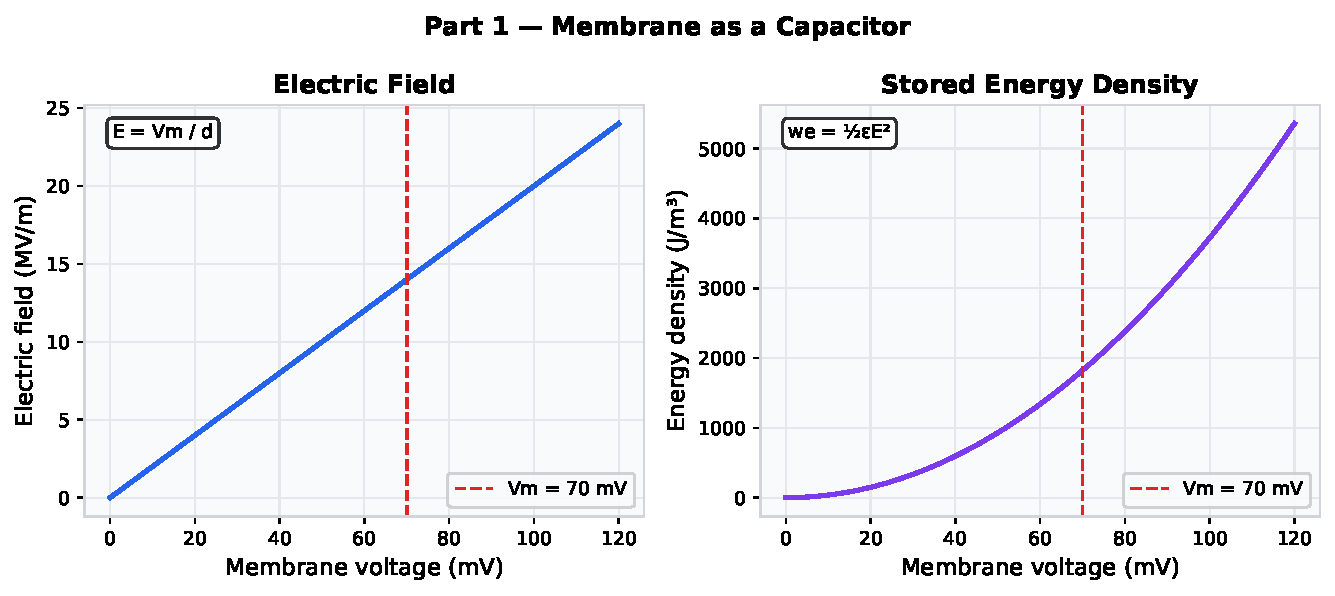
\includegraphics[width=0.92\linewidth]{fig1_membrane.pdf}
  \caption{Left: electric field inside the membrane as a function of
    membrane voltage. Right: electrostatic energy density stored in
    the membrane. Both increase with voltage according to the
    parallel-plate capacitor model.}
  \label{fig:membrane}
\end{figure}

The specific capacitance (per unit area) is $C_m = \varepsilon / d$.
For a lipid membrane with $\varepsilon_r \approx 2.1$ and $d = 5$~nm,
this gives approximately $0.37\;\mu$F/cm$^2$, of the same order as
the commonly used membrane capacitance of $1\;\mu$F/cm$^2$.

% ----------------------------------------------------------
%  3. ACTION POTENTIAL
% ----------------------------------------------------------
\section{The Action Potential}

\subsection{Why a Passive Cable Is Not Enough}

A passive RC cable attenuates voltage as the signal travels. To
transmit a signal over long distances without continuous decay,
neurons use
\emph{voltage-gated ion channels} --- protein pores in the membrane
that open or close depending on the local voltage.

When the membrane voltage exceeds a threshold, sodium (Na$^+$)
channels open and inward sodium current further depolarises the
membrane. This positive feedback produces a rapid spike. Potassium
(K$^+$) channels activate more slowly and repolarise the membrane.
The result is an
\emph{action potential}: a self-regenerating pulse that travels along
the axon without decaying.

\subsection{The Hodgkin--Huxley Model}

Hodgkin and Huxley formulated a quantitative membrane-current model
from voltage-clamp measurements of the squid giant axon
\cite{Hodgkin1952}. Applying KCL at the membrane balances an external
stimulus current with sodium, potassium, and leakage currents:

\begin{formulabox}
\[
  C_m\,\frac{dV}{dt}
    = I_{\text{ext}}
      - \underbrace{\bar{g}_{Na}\,m^3 h\,(V - E_{Na})}_{I_{Na}}
      - \underbrace{\bar{g}_K\,n^4\,(V - E_K)}_{I_K}
      - \underbrace{g_L\,(V - E_L)}_{I_L}
\]
\end{formulabox}

The variables $m$, $h$, and $n$ are dimensionless gating variables
between 0 and 1 that represent channel activation or inactivation.
Each follows a first-order kinetic equation; for example,
\[
  \frac{dm}{dt} = \alpha_m(V)\,(1-m) - \beta_m(V)\,m
\]
The voltage-dependent rate functions $\alpha$ and $\beta$ make the
system nonlinear and enable regenerative spike generation.

\begin{table}[H]
  \centering
  \caption{Hodgkin--Huxley model parameters used in the simulation.}
  \renewcommand{\arraystretch}{1.3}
  \begin{tabular}{llll}
    \toprule
    \textbf{Parameter} & \textbf{Symbol} & \textbf{Value}
      & \textbf{Meaning} \\
    \midrule
    Membrane capacitance   & $C_m$          & $1\;\mu$F/cm$^2$
      & Charge storage \\
    Max Na$^+$ conductance & $\bar{g}_{Na}$ & $120\;$mS/cm$^2$
      & Na$^+$ channel strength \\
    Max K$^+$ conductance  & $\bar{g}_{K}$  & $36\;$mS/cm$^2$
      & K$^+$ channel strength \\
    Na$^+$ reversal pot.   & $E_{Na}$       & $+50\;$mV
      & Na$^+$ equilibrium \\
    K$^+$ reversal pot.    & $E_K$          & $-77\;$mV
      & K$^+$ equilibrium \\
    \bottomrule
  \end{tabular}
  \label{tab:hh}
\end{table}

\begin{figure}[H]
  \centering
  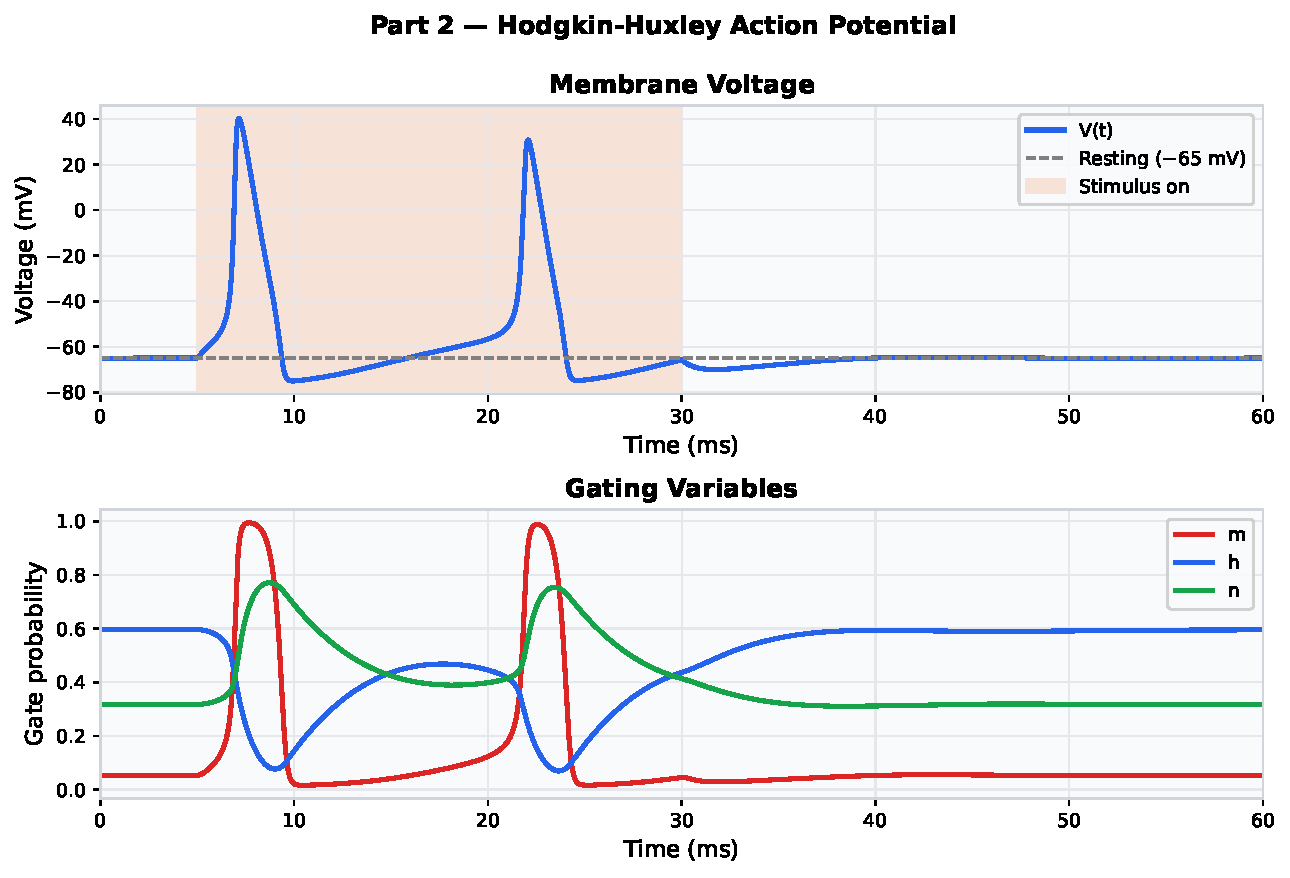
\includegraphics[width=\linewidth]{fig2_hh.pdf}
  \caption{Hodgkin--Huxley simulation at a single point on the membrane.
    Top: membrane voltage --- action potentials fire repeatedly while
    the stimulus current is applied. Bottom: the three gating variables
    $m$, $h$, $n$ showing how the ion channels open and close during
    each spike.}
  \label{fig:hh}
\end{figure}

In Figure~\ref{fig:hh}, $m$ rises sharply at the start of each spike
(Na$^+$ channels opening) and $h$ drops shortly after (Na$^+$ channels
inactivating), while $n$ rises more slowly (K$^+$ channels pulling the
voltage back down). The spike fires again once the channels have reset.

% ----------------------------------------------------------
%  4. PROPAGATION
% ----------------------------------------------------------
\section{Propagation Along the Axon}

\subsection{The Cable Model}

The axon is divided into compartments. Each compartment has an HH
membrane with capacitance and ion channels, while adjacent
compartments are coupled by the axial resistance of the intracellular
fluid. For an axon of radius $a$ and intracellular conductivity
$\sigma_i$, the axial resistance per unit length is
\[
  r_i = \frac{1}{\sigma_i\,\pi a^2}
\]
Defining the intracellular resistivity as $R_i=1/\sigma_i$, the
continuous-limit membrane voltage obeys

\begin{formulabox}
\[
  C_m\,\frac{\partial V}{\partial t}
    = \frac{a}{2R_i}\,\frac{\partial^2 V}{\partial x^2}
      + I_{HH}(V,\,m,\,h,\,n)
\]
\end{formulabox}

where $I_{HH}$ is the net applied and ionic membrane-current density.
This is the classical neuronal cable equation with a nonlinear source
term supplied by the voltage-gated ion channels. Its passive cable
foundation follows the electrotonic framework developed for neurons
and dendritic trees by Rall \cite{Rall1959}.

\subsection{Simulation Result}

A brief current pulse was injected at the left end of a 60~mm model
axon with radius $50\;\mu$m, and the membrane voltage was tracked
across all compartments over time.

\begin{figure}[H]
  \centering
  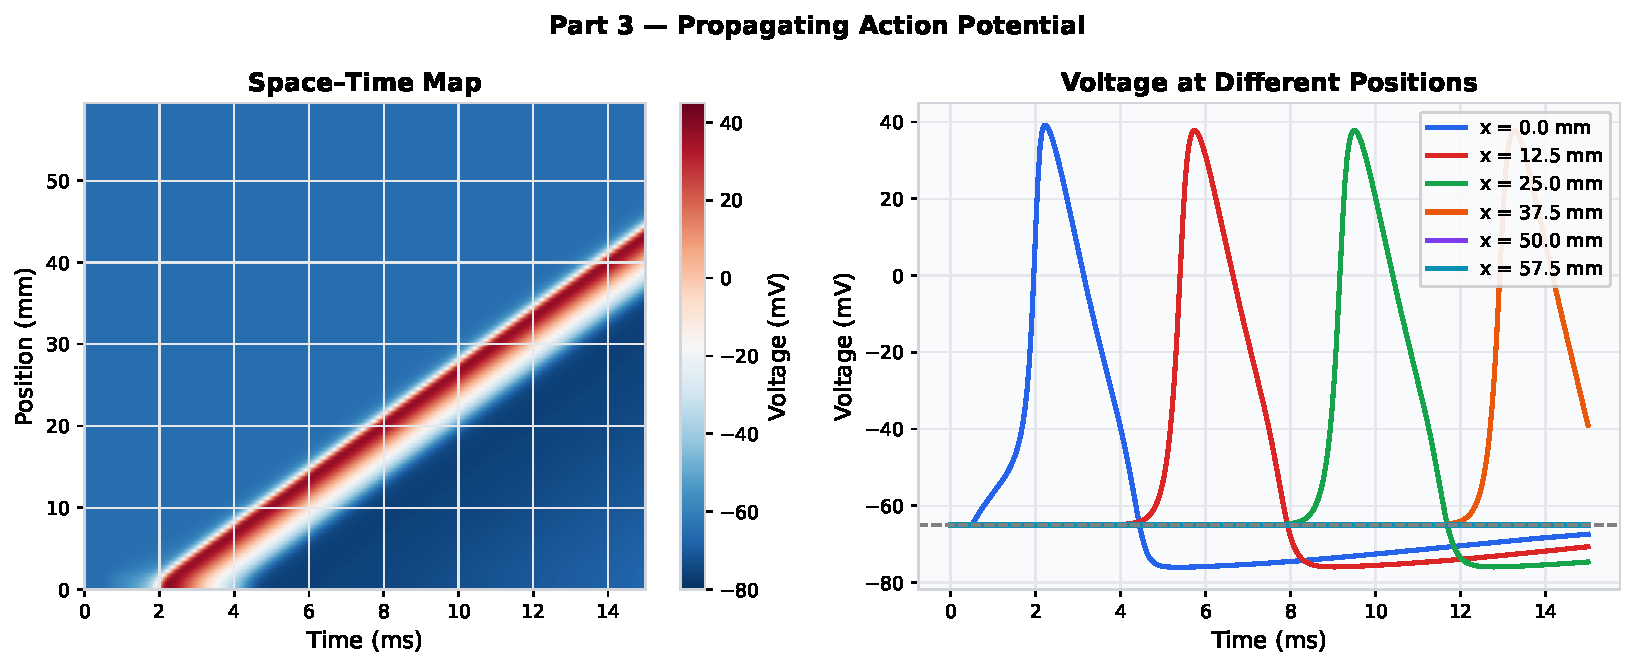
\includegraphics[width=\linewidth]{fig3_propagation.pdf}
  \caption{Action potential propagating along the axon. Left:
    space-time heatmap --- the red band is the action potential
    traveling from left to right at roughly constant speed. Right:
    voltage traces at six positions show the same spike arriving
    later at each successive point.}
  \label{fig:propagation}
\end{figure}

Unlike a passive cable where the signal would decay, here the spike
keeps its shape and amplitude along the full length. The ion channels
at each compartment regenerate the signal locally, so the pulse is
self-sustaining.

For an unmyelinated axon, conduction speed scales approximately as
$\theta \propto \sqrt{a}$: increasing the radius reduces axial
resistance, allowing depolarisation to spread farther ahead and
trigger the next compartment sooner. Myelination increases effective
membrane resistance and decreases capacitance, enabling faster
saltatory conduction between nodes of Ranvier.

\subsection{Assumptions and Limitations}

The model treats the axon as a straight, uniform cylinder with
homogeneous membrane properties and uses the classical
Hodgkin--Huxley parameters obtained from squid giant axon experiments
\cite{Hodgkin1952}. It neglects branching, variations in ion-channel
density, temperature effects, extracellular voltage gradients, and
myelin. The compartmental approximation also introduces spatial and
temporal discretisation error. Consequently, the simulations support
the electromagnetic interpretation and reproduce qualitative spike
behaviour, but they should not be interpreted as a quantitatively
validated model of every neuron type. More detailed neuronal cable
models can incorporate branching geometry and nonuniform membrane
properties \cite{Rall1959}.

% ----------------------------------------------------------
%  5. CONCLUSION
% ----------------------------------------------------------
\section{Conclusion}

This project demonstrates that standard electromagnetic tools apply
directly to neuronal signalling. The membrane stores charge as a
capacitor, the axon behaves as a lossy cable, and voltage-gated ionic
currents regenerate the action potential as it propagates.

The simulations reproduce the principal qualitative features of the
model: repetitive action potentials under sustained stimulation
(Figure~\ref{fig:hh}), propagation with approximately preserved shape
and amplitude (Figure~\ref{fig:propagation}), and membrane fields
consistent with the capacitor approximation
(Figure~\ref{fig:membrane}). Within the stated assumptions, the
combined capacitor, KCL, and cable models provide a coherent
electromagnetic description of neuronal excitation and propagation.

% ----------------------------------------------------------
%  REFERENCES
% ----------------------------------------------------------
\newpage
\bibliographystyle{IEEEtran}
\bibliography{refs}

\end{document}
